\documentclass[UTF8,openany,zihao=-4,oneside]{ctexbook}

% Page and typography
\usepackage[a4paper,top=23mm,bottom=24mm,left=24mm,right=24mm,headheight=15pt,headsep=8mm,footskip=12mm]{geometry}
\linespread{1.08}
\raggedbottom
\sloppy
\emergencystretch=3em

% Core packages
\usepackage{amsmath,amssymb,mathtools}
\usepackage{graphicx}
\graphicspath{{figures/}}
\usepackage{booktabs,longtable,array,tabularx,multirow,makecell}
\usepackage{enumitem}
\usepackage[table]{xcolor}
\usepackage{tikz}
\usetikzlibrary{positioning,arrows.meta,calc,fit,shapes.geometric}
\usepackage{caption}
\usepackage{float}
\usepackage{fancyhdr}
\usepackage{titlesec}
\usepackage{titletoc}
\usepackage{tocloft}
\usepackage[most]{tcolorbox}
\usepackage{listings}
\usepackage{etoolbox}
\usepackage{hyperref}
\usepackage{bookmark}

% Brand colors
\definecolor{FGBlue}{HTML}{1F4E79}
\definecolor{FGDeep}{HTML}{102A43}
\definecolor{FGCyan}{HTML}{2E8BC0}
\definecolor{FGOrange}{HTML}{D98A15}
\definecolor{FGGray}{HTML}{F3F6F9}
\definecolor{FGLine}{HTML}{D7E2EA}
\definecolor{FGText}{HTML}{243B53}

\hypersetup{
  colorlinks=true,
  linkcolor=FGBlue,
  urlcolor=FGCyan,
  citecolor=FGOrange,
  pdfauthor={FlameGuard},
  pdftitle={稳燃宝垃圾脱水实验设计手册},
  pdfsubject={垃圾干燥脱水实验、数据采集、干燥特性分析},
  pdfkeywords={FlameGuard, 稳燃宝, 垃圾脱水, 干燥实验, 含水率, 预热控制}
}

% Paragraph and list tuning
\setlength{\parindent}{2em}
\setlength{\parskip}{0.18em}
\setlist{itemsep=0.15em,topsep=0.35em,leftmargin=2.2em}
\renewcommand{\arraystretch}{1.22}
\setlength{\tabcolsep}{5pt}
\setlength{\LTleft}{0pt}
\setlength{\LTright}{0pt}
\AtBeginEnvironment{longtable}{\small\renewcommand{\arraystretch}{1.2}}

% Utilities
\providecommand{\tightlist}{\setlength{\itemsep}{0pt}\setlength{\parskip}{0pt}}
\providecommand{\passthrough}[1]{#1}
\newcommand{\manualdivider}{\par\vspace{0.6em}\noindent\textcolor{FGLine}{\rule{\linewidth}{0.7pt}}\vspace{0.6em}\par}
\newcommand{\notebox}[2]{\begin{tcolorbox}[enhanced,colback=FGBlue!4,colframe=FGBlue!45,boxrule=0.5pt,arc=1.5mm,left=4mm,right=4mm,top=3mm,bottom=3mm]\sffamily\textbf{\color{FGDeep}#1}\par\vspace{0.25em}\color{FGText}#2\end{tcolorbox}}
\newcommand{\warnbox}[2]{\begin{tcolorbox}[enhanced,colback=FGOrange!6,colframe=FGOrange!55,boxrule=0.5pt,arc=1.5mm,left=4mm,right=4mm,top=3mm,bottom=3mm]\sffamily\textbf{\color{FGDeep}#1}\par\vspace{0.25em}\color{FGText}#2\end{tcolorbox}}

% Captions
\captionsetup{font=small,labelfont={bf,color=FGBlue},labelsep=quad}

% Chapter / section styles
\titleformat{\chapter}[display]
  {\Huge\bfseries\sffamily\color{FGDeep}}
  {\begin{tikzpicture}[baseline=(n.base)]\node[fill=FGBlue,text=white,rounded corners=1.5mm,inner xsep=8pt,inner ysep=5pt,font=\Large\bfseries\sffamily] (n) {第\thechapter 章};\end{tikzpicture}}
  {0.85em}
  {\Huge}
  [\vspace{0.35em}{\color{FGOrange}\titlerule[1.2pt]}]
\titlespacing*{\chapter}{0pt}{-4mm}{11mm}

\titleformat{\section}
  {\Large\bfseries\sffamily\color{FGBlue}}
  {\thesection}{0.75em}{}
  [\vspace{0.15em}{\color{FGLine}\titlerule[0.6pt]}]
\titlespacing*{\section}{0pt}{2.1ex plus .4ex}{1.1ex}

\titleformat{\subsection}
  {\large\bfseries\sffamily\color{FGDeep}}
  {\thesubsection}{0.75em}{}
\titlespacing*{\subsection}{0pt}{1.8ex plus .3ex}{0.8ex}

\titleformat{\subsubsection}
  {\normalsize\bfseries\sffamily\color{FGDeep}}
  {\thesubsubsection}{0.65em}{}
\titlespacing*{\subsubsection}{0pt}{1.3ex plus .2ex}{0.55ex}

% TOC styling
\renewcommand{\cftchapfont}{\sffamily\bfseries\color{FGDeep}}
\renewcommand{\cftsecfont}{\sffamily\color{FGText}}
\renewcommand{\cftchappagefont}{\sffamily\bfseries\color{FGBlue}}
\renewcommand{\cftsecpagefont}{\sffamily\color{FGText}}
\setlength{\cftbeforechapskip}{0.45em}

% Header / footer
\pagestyle{fancy}
\fancyhf{}
\fancyhead[L]{\sffamily\small\color{FGDeep}“稳燃宝”垃圾脱水实验设计手册}
\fancyhead[R]{\sffamily\small\color{FGBlue}\leftmark}
\fancyfoot[L]{\sffamily\scriptsize\color{FGText}实验装置 · 样品工况 · 干燥曲线 · 结果分析}
\fancyfoot[R]{\sffamily\small\bfseries\color{FGBlue}\thepage}
\renewcommand{\headrulewidth}{0.5pt}
\renewcommand{\footrulewidth}{0pt}
\renewcommand{\headrule}{\hbox to\headwidth{\color{FGLine}\leaders\hrule height \headrulewidth\hfill}}
\fancypagestyle{plain}{%
  \fancyhf{}%
  \fancyfoot[R]{\sffamily\small\bfseries\color{FGBlue}\thepage}%
  \renewcommand{\headrulewidth}{0pt}%
}

% Code listings
\lstdefinestyle{fgcode}{
  basicstyle=\ttfamily\small,
  backgroundcolor=\color{FGGray},
  frame=single,
  rulecolor=\color{FGLine},
  framerule=0.5pt,
  breaklines=true,
  columns=fullflexible,
  keepspaces=true,
  showstringspaces=false,
  tabsize=2,
  xleftmargin=1em,
  xrightmargin=1em,
  framexleftmargin=0.6em,
  framexrightmargin=0.6em,
  aboveskip=0.8em,
  belowskip=0.8em
}
\lstset{style=fgcode}

\newcommand{\fgbadge}[1]{\tcbox[colback=FGBlue!6,colframe=FGBlue!35,boxrule=0.4pt,arc=1mm,left=2pt,right=2pt,top=1pt,bottom=1pt,on line]{\sffamily\footnotesize #1}}

\begin{document}

\begin{titlepage}
\begin{tikzpicture}[remember picture,overlay]
  \fill[FGDeep] (current page.north west) rectangle ([yshift=-88mm]current page.north east);
  \fill[FGBlue] ([yshift=-88mm]current page.north west) rectangle ([yshift=-92mm]current page.north east);
  \fill[FGOrange] ([yshift=-92mm]current page.north west) rectangle ([yshift=-94mm]current page.north east);
  \fill[FGGray] ([yshift=-94mm]current page.north west) rectangle (current page.south east);
  \draw[FGBlue!20,line width=1.2pt] ([xshift=18mm,yshift=-122mm]current page.north west) -- ([xshift=-18mm,yshift=-122mm]current page.north east);
\end{tikzpicture}
\vspace*{13mm}
{\sffamily\bfseries\color{white}\fontsize{18}{22}\selectfont FlameGuard / 稳燃宝}\par
\vspace{9mm}
{\sffamily\bfseries\color{white}\fontsize{33}{40}\selectfont 垃圾脱水实验设计手册}\par
\vspace{4mm}
{\sffamily\color{white}\fontsize{15}{20}\selectfont 样品制备 · 连续称重 · 干燥曲线 · 结果分析}\par
\vspace{36mm}
\begin{tcolorbox}[enhanced,width=\textwidth,colback=white,colframe=FGLine,boxrule=0.7pt,arc=2mm,drop shadow={black!12!white},left=8mm,right=8mm,top=6mm,bottom=6mm]
{\sffamily\bfseries\Large\color{FGDeep}v0.2.0 Beta}\par\vspace{0.6em}
\end{tcolorbox}
\vfill
{\sffamily\small\color{FGText}炉火纯青队 · 大学生节能减排社会实践与科技竞赛 · 2025}\par
\end{titlepage}

\frontmatter
\pagestyle{plain}
\tableofcontents
\cleardoublepage
\pagestyle{fancy}
\mainmatter

\chapter{概述}

\section{实验目的}

小型垃圾焚烧设施面对高湿、低热值入料时，容易出现炉膛温度波动、辅助燃料消耗增加和燃烧不稳定等问题。垃圾脱水实验用于获得典型生活垃圾在不同加热温度下的含水率变化规律，为预热条件设定提供基础数据。

本实验重点回答三类问题：
\begin{enumerate}
\item 不同垃圾组分的初始湿基含水率差异；
\item 不同加热温度下垃圾含水率随时间的变化规律；
\item 达到目标含水率所需时间与垃圾组分、加热温度之间的关系。
\end{enumerate}

\notebox{实验定位}{实验结果用于建立垃圾组分占比、预热条件和脱水效果之间的对应关系，支撑预热系统对烟气温度、烟气流速和停留时间的设定。}

\section{实验对象}

实验对象选取乡村生活垃圾中占比较高、对焚烧稳定性影响较大的厨余类组分，包括菜叶、西瓜皮、橘子皮、米饭、肉类，并设置混合样进行验证。混合样按菜叶 30\%、西瓜皮 20\%、橘子皮 10\%、米饭 25\%、肉类 15\% 的质量占比配置。

\begin{table}[htbp]
\centering
\begin{tabularx}{0.86\textwidth}{p{30mm}p{28mm}X}
\toprule
组分 & 质量占比 & 说明 \\
\midrule
菜叶 & 30\% & 高湿叶菜类组分。\\
西瓜皮 & 20\% & 高湿果皮类组分。\\
橘子皮 & 10\% & 果皮类组分。\\
米饭 & 25\% & 淀粉类熟食组分。\\
肉类 & 15\% & 蛋白/脂肪类组分，初始含水率相对较低。\\
\bottomrule
\end{tabularx}
\caption{典型混合样质量配比}
\label{tab:mix-ratio}
\end{table}

\section{实验输出}

实验输出包括连续称重数据、湿基含水率曲线、到达指定含水率所需时间和不同温度下的脱水速率差异。建模主要使用以下指标：
\begin{enumerate}
\item 初始净重 $m_0$ 和结束净重 $m_d$；
\item 初始湿基含水率 $\omega_0$；
\item 达到 0\% 含水率和 52.35\% 含水率的时间；
\item 组分差异、干燥速度差异和温度响应差异。
\end{enumerate}

\manualdivider

\chapter{实验设计}

\section{实验装置}

实验系统由台式烘箱、在线电子天平、挂钩/托盘连接结构和数据采集电脑组成。烘箱提供恒温加热环境，电子天平通过挂钩与烘箱内托盘连接，在不取出样品的情况下连续记录质量变化。数据采集电脑实时保存质量--时间序列。

\begin{figure}[htbp]
\centering
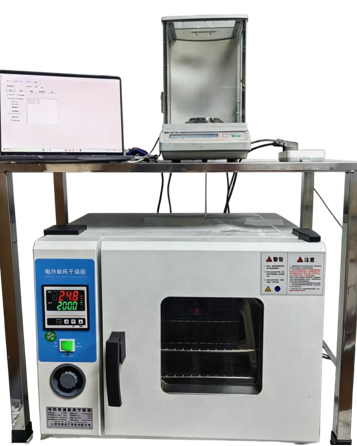
\includegraphics[width=0.78\textwidth]{fig_experiment_setup.png}
\caption{实验装置现场图}
\label{fig:experiment-setup}
\end{figure}

\begin{table}[htbp]
\centering
\begin{tabularx}{\textwidth}{p{30mm}p{40mm}X}
\toprule
模块 & 参数或配置 & 作用 \\
\midrule
台式烘箱 & 控温精度约 0.1\,\textdegree C & 提供恒温干燥环境。\\
在线电子天平 & 精度 0.001\,g & 连续记录样品质量变化。\\
挂钩与托盘 & 连接天平与烘箱内样品 & 保证加热过程与称重过程同步进行。\\
数据采集电脑 & 与电子天平连接 & 实时采集、传输和保存称重数据。\\
\bottomrule
\end{tabularx}
\caption{实验系统组成}
\label{tab:equipment}
\end{table}

\begin{figure}[htbp]
\centering
\begin{minipage}{0.47\textwidth}
\centering
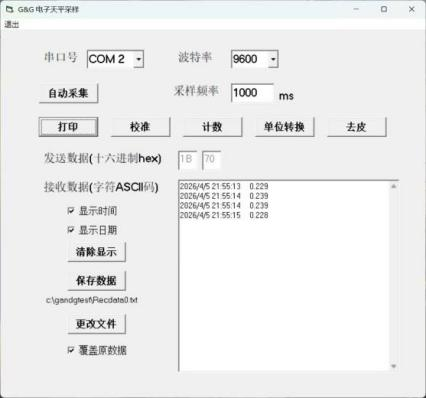
\includegraphics[width=\textwidth]{fig_balance_ui.jpeg}
\end{minipage}\hfill
\begin{minipage}{0.47\textwidth}
\centering
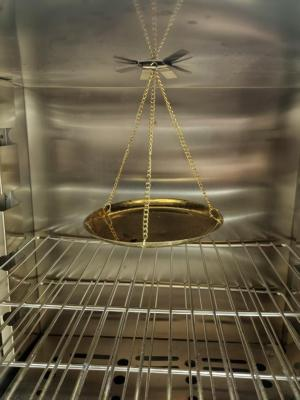
\includegraphics[width=\textwidth]{fig_oven_inside.jpeg}
\end{minipage}
\caption{电子天平数据采集界面（左）与烘箱内部安装图（右）}
\label{fig:balance-and-oven}
\end{figure}

\section{实验工况}

实验采用控制变量法，以加热温度和加热时间为核心变量。基础温度梯度为 125\,\textdegree C、150\,\textdegree C、175\,\textdegree C；实验数据中同时记录了 200\,\textdegree C 以及米饭 215\,\textdegree C 的补充工况，用于观察升温后的脱水加速趋势。

\begin{table}[htbp]
\centering
\begin{tabularx}{\textwidth}{p{32mm}p{42mm}X}
\toprule
变量类别 & 设置 & 说明 \\
\midrule
垃圾组分 & 菜叶、西瓜皮、橘子皮、米饭、肉类、混合样 & 覆盖高湿植物类、果皮类、淀粉类和肉类组分。\\
加热温度 & 125、150、175、200、215\,\textdegree C & 用于比较不同加热强度下的脱水速度。\\
加热时间 & 至质量趋于稳定或达到目标含水率 & 由连续称重曲线确定关键时间点。\\
重复次数 & 每组实验重复 3 次取平均值 & 降低偶然误差。\\
输出指标 & 含水率、到 0\% 含水率时间、到 52.35\% 含水率时间 & 用于干燥特性分析和参数匹配。\\
\bottomrule
\end{tabularx}
\caption{脱水实验变量设置}
\label{tab:variables}
\end{table}

\begin{figure}[htbp]
\centering
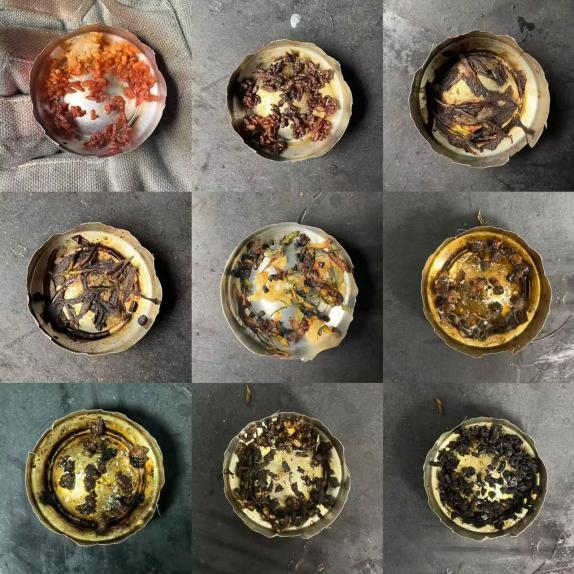
\includegraphics[width=0.76\textwidth]{fig_field_samples.jpeg}
\caption{部分现场实验样品记录}
\label{fig:field-samples}
\end{figure}

\section{实验流程}

每个“组分--温度”组合按统一流程执行：
\begin{enumerate}
\item 将样品切分为尺寸接近的小块，称量初始净重 $m_0$；
\item 将烘箱升至目标温度并保持稳定；
\item 安装托盘和挂钩，确认天平读数稳定；
\item 放入样品，关闭烘箱门，启动数据采集；
\item 连续记录样品质量 $m(t)$，直到质量变化趋于平缓或达到实验终止条件；
\item 记录结束净重 $m_d$，保存原始数据和处理结果；
\item 同一工况重复实验并取平均值。
\end{enumerate}

\section{数据处理方法}

湿基含水率按式 \eqref{eq:wet-basis-moisture} 计算：
\begin{equation}
\omega(t)=\frac{m(t)-m_d}{m(t)}\times 100\% .
\label{eq:wet-basis-moisture}
\end{equation}

初始湿基含水率按式 \eqref{eq:initial-moisture} 计算：
\begin{equation}
\omega_0=\frac{m_0-m_d}{m_0}\times 100\% .
\label{eq:initial-moisture}
\end{equation}

水分去除率可按式 \eqref{eq:removal-ratio} 计算：
\begin{equation}
\eta(t)=\frac{m_0-m(t)}{m_0-m_d}\times 100\% .
\label{eq:removal-ratio}
\end{equation}

当 $\eta(t)=80\%$ 时，对应时间记为 $t_{80}$，用于比较不同组分的脱水速度。对于不同温度下的干燥时间，可用线性近似描述温度响应：
\begin{equation}
 t_i(T)=t_{ref,i}+s_i\left(T-T_{ref}\right),
\label{eq:temperature-sensitivity}
\end{equation}
其中 $i$ 表示垃圾组分，$T_{ref}$ 为参考温度，$t_{ref,i}$ 为参考温度下达到目标脱水程度所需时间，$s_i$ 为温度敏感性系数。

\manualdivider

\chapter{实验结果}

\section{实验数据表}

{\scriptsize
\setlength{\tabcolsep}{2pt}
\begin{longtable}{@{}p{15mm}p{14mm}p{18mm}p{18mm}p{20mm}p{24mm}p{27mm}@{}}
\caption{不同组分生活垃圾干燥特性实验结果}\label{tab:raw-results}\\
\toprule
\makecell{垃圾\\组分} & \makecell{实验\\温度/\textdegree C} & \makecell{初始\\净重/g} & \makecell{结束\\净重/g} & \makecell{湿基\\含水率/\%} & \makecell{到 0\% 含水率\\时间/min} & \makecell{到 52.35\% 含水率\\时间/min} \\
\midrule
\endfirsthead
\toprule
\makecell{垃圾\\组分} & \makecell{实验\\温度/\textdegree C} & \makecell{初始\\净重/g} & \makecell{结束\\净重/g} & \makecell{湿基\\含水率/\%} & \makecell{到 0\% 含水率\\时间/min} & \makecell{到 52.35\% 含水率\\时间/min} \\
\midrule
\endhead
橘子皮 & 150 & 7.867 & 1.492 & 81.03 & 32.88 & 18.88 \\
橘子皮 & 175 & 8.070 & 1.464 & 81.86 & 26.90 & 14.26 \\
橘子皮 & 200 & 7.703 & 1.369 & 82.23 & 17.08 & 10.54 \\
米饭 & 150 & 11.562 & 4.698 & 59.37 & 45.90 & 8.59 \\
米饭 & 175 & 9.569 & 3.601 & 62.37 & 28.40 & 7.29 \\
米饭 & 200 & 10.153 & 3.893 & 61.66 & 24.67 & 5.60 \\
米饭 & 215 & 8.656 & 3.375 & 61.01 & 16.83 & 3.60 \\
肉类 & 125 & 7.022 & 4.568 & 34.95 & 46.13 & 0.00 \\
肉类 & 150 & 5.969 & 3.415 & 42.79 & 23.03 & 0.00 \\
肉类 & 175 & 6.098 & 3.180 & 47.85 & 17.95 & 0.00 \\
肉类 & 200 & 5.864 & 2.853 & 51.35 & 17.57 & 0.00 \\
菜叶 & 125 & 5.112 & 0.366 & 92.84 & 31.87 & 22.60 \\
菜叶 & 150 & 3.885 & 0.185 & 95.24 & 22.10 & 16.23 \\
菜叶 & 175 & 5.183 & 0.124 & 97.61 & 21.48 & 19.06 \\
菜叶 & 200 & 4.687 & 0.300 & 93.60 & 13.47 & 9.85 \\
西瓜皮 & 150 & 8.694 & 0.476 & 94.52 & 43.50 & 32.63 \\
西瓜皮 & 175 & 8.925 & 0.509 & 94.30 & 31.28 & 22.84 \\
西瓜皮 & 200 & 8.932 & 0.398 & 95.54 & 22.65 & 17.32 \\
混合样 & 150 & 10.137 & 2.232 & 77.98 & 40.82 & 19.14 \\
混合样 & 175 & 10.006 & 2.319 & 76.82 & 30.13 & 13.19 \\
混合样 & 200 & 9.976 & 2.290 & 77.04 & 24.10 & 10.29 \\
\bottomrule
\end{longtable}
}

\section{干燥曲线}

不同温度下的干燥曲线显示，垃圾含水率随加热时间延长呈先快速下降、后趋于平缓的变化规律。加热温度越高，脱水速率越快，达到同一目标含水率所需时间越短。

\begin{figure}[htbp]
\centering
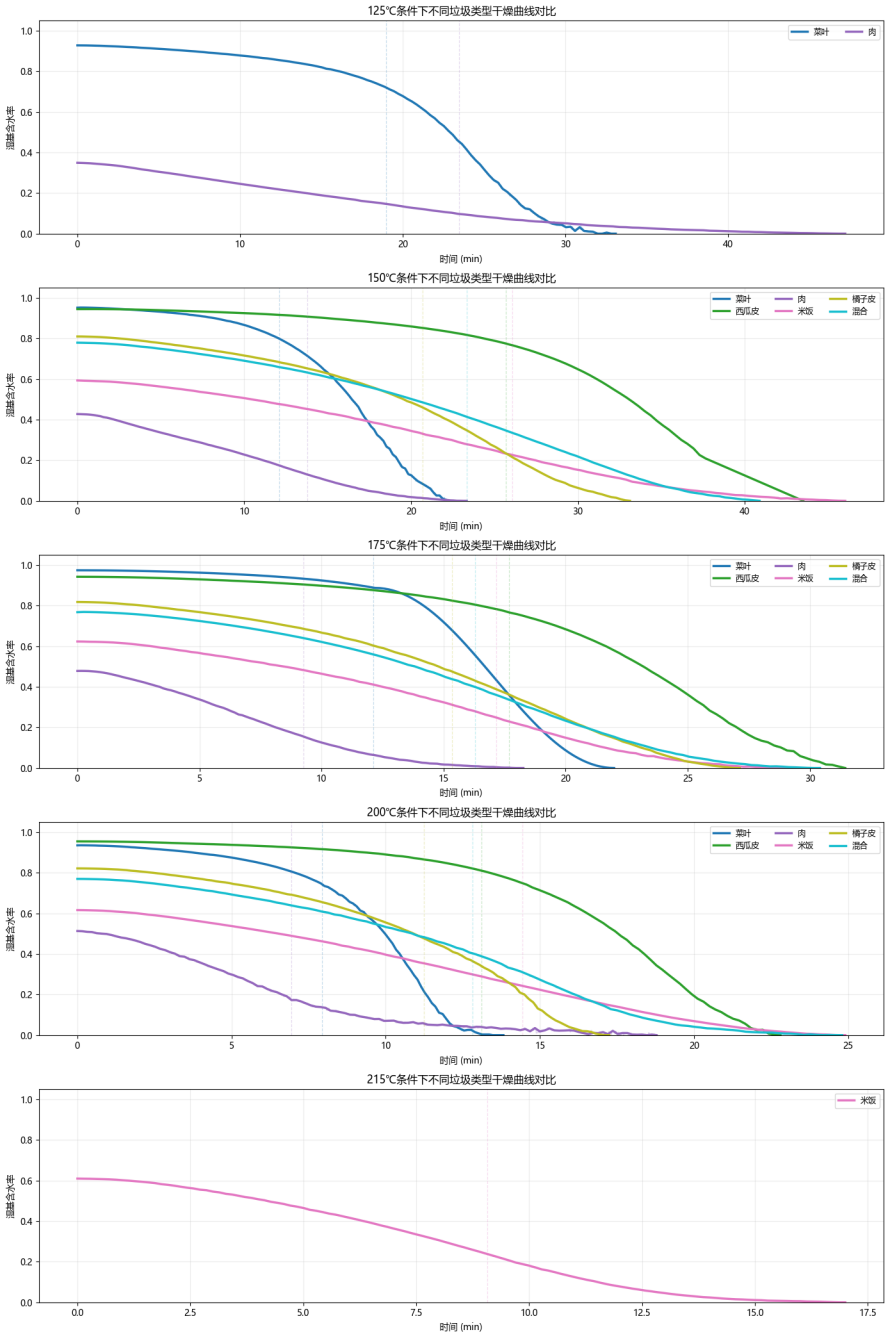
\includegraphics[width=0.76\textwidth]{fig_drying_curves_temperature.png}
\caption{各温度下不同种类垃圾干燥曲线对比}
\label{fig:drying-curves-temperature}
\end{figure}

\begin{figure}[htbp]
\centering
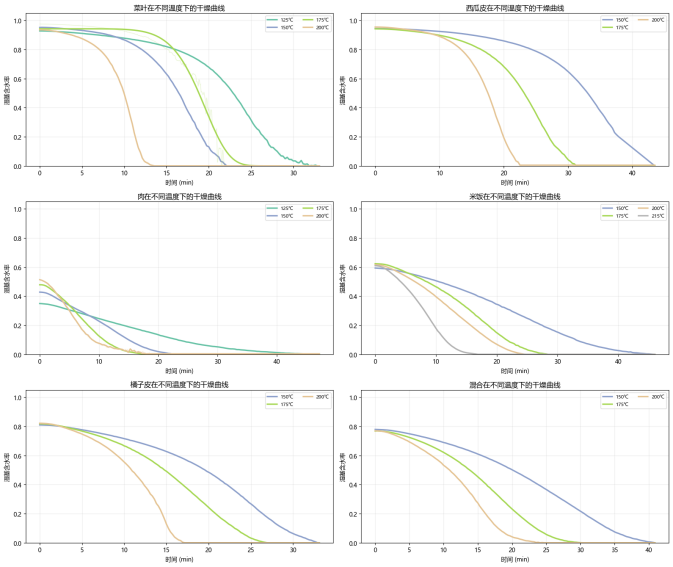
\includegraphics[width=0.86\textwidth]{fig_drying_curves_groups.png}
\caption{各实验组干燥特性曲线}
\label{fig:drying-curves-groups}
\end{figure}

\section{干燥特性参数}

从实验结果可提取初始湿基含水率 $\omega_i$、参考干燥时间 $t_{ref,i}$ 和温度敏感性系数 $s_i$。参数整理如下：

\begin{table}[htbp]
\centering\footnotesize
\begin{tabularx}{\textwidth}{p{16mm}p{20mm}p{28mm}p{44mm}X}
\toprule
组分编号 & 组分名称 & 初始湿基含水率 $\omega_i$ & 175\,\textdegree C 下 20\% 含水率干燥时间 $t_{ref,i}$/min & 温度敏感性系数 $s_i$/(min/\textdegree C) \\
\midrule
$x_1$ & 菜叶 & 0.948 & 12.1 & -0.132 \\
$x_2$ & 西瓜皮 & 0.948 & 17.7 & -0.251 \\
$x_3$ & 橘子皮 & 0.817 & 15.3 & -0.189 \\
$x_4$ & 肉类 & 0.442 & 11.5 & -0.216 \\
$x_5$ & 混合样 & 0.773 & 16.3 & -0.210 \\
$x_6$ & 米饭 & 0.611 & 15.8 & -0.243 \\
\bottomrule
\end{tabularx}
\caption{典型厨余垃圾干燥特性参数}
\label{tab:kinetic-param}
\end{table}

\begin{figure}[htbp]
\centering
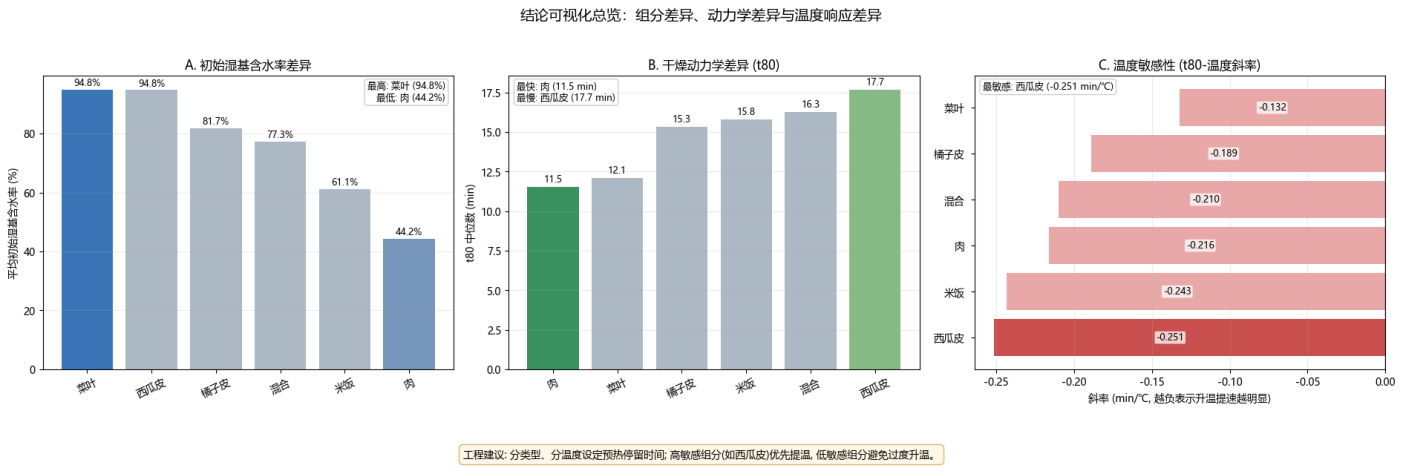
\includegraphics[width=0.92\textwidth]{fig_conclusion_analysis.png}
\caption{结论可视化分析：组分差异、动力学差异与温度响应差异}
\label{fig:conclusion-analysis}
\end{figure}

\section{结果分析}

实验结果表明，不同垃圾组分的初始湿基含水率差异明显。菜叶平均初始湿基含水率最高，约为 94.8\%；肉类样品相对较低，约为 44.2\%。该差异说明预热控制不能只采用单一含水率假设，而应考虑组分构成。

从干燥动力学看，各类垃圾达到 80\% 去除率所需时间存在差异。按 $t_{80}$ 中位数统计，肉类样品干燥速度最快，$t_{80}$ 为 11.5\,min；西瓜皮样品最慢，$t_{80}$ 为 17.7\,min。

从温度响应看，升温总体上能够加快干燥过程，但不同组分响应强度不同。西瓜皮对温度最敏感，$t_{80}$--温度斜率为 -0.251\,min/\textdegree C；菜叶温度敏感性相对较弱。工程应用中应采用分组分、分温度的脱水策略，以减少预热不足或过度预热。

\end{document}
